\documentclass[11pt,twoside]{rmta2010esp}% For English, use rmta2010eng.cls instead of rmta2010esp.cls
%\pagestyle{myheadings} 
\usepackage[english, spanish]{babel}
\usepackage{fancyhdr}
\usepackage[utf8]{inputenc} % En caso de usar tildes, ñ y otros caracteres especiales



\pagestyle{fancy}
\fancyhead{}
\fancyhead[RE]{\thepage \hfill {\sc a. rib\'{o} -- g. molina -- r. r\'{i}os  }}
\fancyhead[LO]{{\sc Combining neural networks and geostatistics for landslide hazard assessment of San Salvador Metropolitan Area, El Salvador } \hfill \thepage}
\fancyfoot{}
\fancyfoot[RE]{{\scriptsize{\it Rev.Mate.Teor.Aplic.} (ISSN 1409-2433) {Vol. 19}(1): 1--10, January 2012}}
\fancyfoot[LO]{{\scriptsize{\it Rev.Mate.Teor.Aplic.} (ISSN 1409-2433) {Vol. 19}(1): 1--10, January 2012}}
\paginas{1}{10} % Numeros de pgina, la versión final la pone el editor; Page numbers, the Editor puts the final numbers
\usepackage{amsmath}
\usepackage{amssymb}
\usepackage{graphics}
\usepackage{graphicx} % En caso de usar figuras, con formato .esp; In case of using figures, with format .eps
\usepackage{float} 
\usepackage{url}
\usepackage{amsfonts}
\usepackage{amsmath}
\usepackage{enumerate}
\usepackage{authblk}
\usepackage{hyperref}


\DeclareGraphicsExtensions{.bmp,.png,.pdf,.jpg,.eps}



\renewcommand{\refname}{References} 



\begin{document}

\selectlanguage{spanish}
\title{Combining neural networks and geostatistics for landslide hazard assessment of San Salvador Metropolitan Area, El Salvador 
\newline
\newline
Combinando redes neuronales y geoestad\'{i}stica para evaluaci\'{o}n de deslizamientos de tierra de el \'{a}rea Metropolitana de San Salvador, El Salvador}

\author[1]{Alex Rib\'{o} \thanks{alexandre4rt@gmail.com }}
\author[2]{Giovanni Molina \thanks{giova.molina@gmail.com}}
\author[3]{Ricardo Ríos \thanks{ricardo.sv@gmail.com}}


\affil[1]{National Institute of Health, Ministry of Health of El Salvador, El Salvador.}
\affil[2]{Ministry of Environment and Natural Resources of El Salvador.}
\affil[3]{Department of Mathematics, Science and Mathematics Faculty, University of El Salvador, El Salvador.}



\maketitle

%\newpage 

\selectlanguage{spanish}
\begin{resumen}
Esta contribución describe la creaci\'{o}n de un modelo de evaluaci\'{o}n de deslizamiento de tierra para San Salvador, departamento de El Salvador. El an\'{a}lisis inicio con la obtenci\'{o}n de una foto área del MARN (Ministerio de Medio Ambiente y Recursos Naturales) con un total de 939407 puntos georeferenciados con el fin de producir un inventario de deslizamiento. En esta evaluaci\'{o}n de los deslizamientos se uso 4792 eventos previamente foto-interpretados y 7 factores condicionantes incluyendo: geomorfolog\'{i}a, geolog\'{i}a, precipitaciones m\'{a}ximas, aceleraciones s\'{i}smicas, pendiente del terreno, distancia a carretera y falla geol\'{o}gica. Redes Neuronales Artificiales(RNA) fueron usadas para la evaluaci\'{o}n de la susceptibilidad a deslizamiento de tierra, logrando que m\'{a}s del 80\% de deslizamientos fueran apropiadamente clasificados usando un criterio dentro y fuera de la muestra con la que se estimaron los parámetros del modelo. Regresi\'{o}n Log\'{i}stica fue usada como base de comparaci\'{o}n, obteniendo este modelo un rendimiento inferior que el de RNA con un porcentaje de correcta clasificaci\'{o}n abajo del 70\%. Para completar el an\'{a}lisis se realizo la interpolaci\'{o}n de puntos usando el m\'{e}todo krigging proveniente del enfoque geoestad\'{i}stico. Finalmente, los resultados muestran que es posible obtener un mapa de riesgo a deslizamiento de tierra, haciendo uso de una combinación de RNA y t\'{e}cnicas geoestad\'{i}sticas con lo cual la presente investigación puede ayudar a la mitigación de deslizamientos de tierra en El Salvador.
\end{resumen}

\PC deslizamiento de tierra, evaluación de riesgo, El Salvador, RNA, geoestadística.

\begin{abstract}
This contribution describes the creation of a landslide hazard
assessment model for San Salvador, department in El Salvador. The analysis started with an aerial photointerpretation from  MARN (Ministry of Environment and Natural Resources of El Salvador)  with a total amount of 939407 georeferenced points to produce a landslide inventory. In this
landslide assessment we have used 4792 events previously photo-interpretaded
and 7 conditioning factors including: geomorphology, geology, rainfall intensity, peak ground accelaration, slope angle, road and fault distance. Artificial
Neural Networks (ANNs) were applied for the assessment of susceptibility to
landslides, achieving more than 80\% of landslide were properly classified using
in-sample and out of sample criteria. Logistic regression was used as base of
comparison, obtaining this model a performance lower than ANNs with a percentage of correct classification under 70\%. To complete the analysis we have
performed interpolation of the points using kriging method from geostatistical
approach. Finally, the results show that is possible to derive a landslide hazard map, making use of a combination of ANNs and geostatistical techniques
wherewith the present study can help landslide mitigation in El Salvador.
\end{abstract}

\KW landslide, hazard assessment, El Salvador, ANN, geostatistics.

\AMS 62P12.% Mathematical Subject Classification, http://www.ams.org/mathscinet/msc/msc2010.html.

\selectlanguage{english}


\section{Introduction}
\label{sec:intr}
El Salvador, one of the smallest and most crowded nations in Central America, extends about 240 kilometers westward from the 
Gulf of Fonseca to the border with Guatemala. This country is very vulnerable to landslide due to social, political and economic factors.
In the year of 2001, El Salvador was struck by two devastating earthquakes within a month. One of the most spectacular aspects featuring 
heavily in the first earthquake was the damage inflicted by landslides. Among them, Las Colinas landslide was the most tragic.
A huge amount of soil mass (about 200,000 $m^{3}$) was thrown off the rim of a mountain ridge rising south behind Las Colinas area 
of Nueva San Salvador (Santa Tecla), and flushed many houses and therefore more than 500 lives to death.

Due to the above it is necessary to implement mechanisms that allow us to quantify the hazard of a given
geographic area to landslides, usually this is done with development of susceptibility maps which present in a graphical way
the zones more susceptible to landslides and represent a practical tool for urban planning.

%% write about how to perform your neural network and geostatistic analysis

%The data was collected from aerial images, topographical and geologic maps which provide a base for  the application of landslide susceptibility methodologies and the development of geostatistics models. From aerial photographs, different regions of landslide occurrences were classified. The topographical and geologic maps provided information about causal factors. 
%
%
%Artificial neural networks (ANNs) are computational models inspired by biology (in particular the brain) that are capable of machine learning and pattern recognition. They are usually presented as systems of interconnected ``neurons'' that can compute values from inputs by feeding information through the network (\citet{wiki:001}). Recently ANNs have been applied successfully to the assessment of landslide susceptibility. 
%
In this paper we propose an ANN model which enable to estimate the susceptibility to landslide in the georeferenced points belong to the Metropolitan Area of San Salvador (MASS) and later a map of susceptibility was generated by means of kriging method from geostatistical. 



%\citet{Melchiorre2011410} determined landslide susceptibility for the Guantanamo Province %in Cuba by using ANN models. 

%%% I must citet the paper of Enrique Castellanos 



\section{Brief State of Art}
\label{sec:brief}
Since the pioneering work (\cite{Carrara1983403}), several mathematics and statistics models have been proposed to model landslide susceptibility: deterministic models (\cite{hessd-10-12643-2013},  \cite{doi:10.1080/19475705.2010.498151} and \cite{Neu2012511}), probabilistic models (\cite{Bern198839}, \cite{Chung2003451} and \cite{doi:10.1080/01431160310001618734} ). 

It has been used popular classification models such as logistic regression (\cite{akgun2012} and \cite{gaskill} ) , neural networks (\cite{Melchiorre2011410},\cite{Zeng2001374}, \cite{Ermini2005327}) and \cite{Yesilnacar2005251} and support vector machine (\cite{ballabio2012support} and \cite{tien2012landslide}). 


According to (\cite{van2006landslide}) the magnitude of a possible
slide is difficult to foresee as it depends on the magnitude of the triggering event and the environmental conditions (e.g., height of water table) at the moment of the event. Because of these complex relationships between the dependent variable and causal factors, and since that neural networks are particularly useful for detect complex non-linear relationships in large datasets, that is why this kind of model was chosen, despite the disadvantages such as greater computational burden and proneness to overfitting.  



%There are two important applications of the neural network models to landslide susceptibility. The first (\cite{Yesilnacar2005251})

%Despite of the recent use of maps in those published works have not given enough attention on the use of geostatistical models to interpolate spatially distributed landslide susceptibility just landslide susceptibility is given in the georeferenced points and showed in the map of susceptibility.

\section{Landslide inventory and data sources of input variables}
\label{sec:landsinvet}
The Landslide inventory was developed from photographic analysis on the study area, using 
aerial photo from MARN which is presented in the Figure \ref{fig:img01}, where white areas represent regions of landslide occurrence which were processed using the software ILWIS. 

 \begin{center}
  \begin{figure}[H]
   \centering
   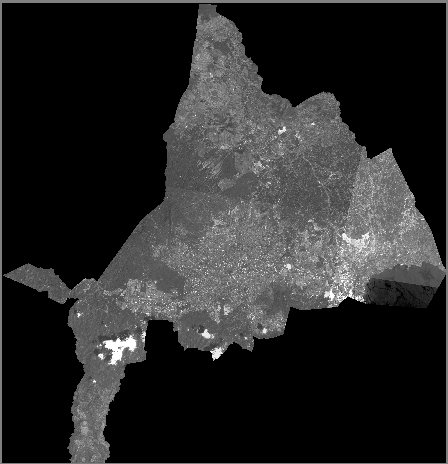
\includegraphics[scale=0.40]{img01}
   \caption{\small{Aerial photo of MASS}}
   \label{fig:img01}
  \end{figure}
 \end{center}

Once that the white areas were georeferenced, a percentage of 0.5\% of the total points georeferenced shows landslide ocurrence. In addition to the landslide information the following data sources of input variables was given by MARN: 
\begin{enumerate}
\item {\bf Geomorphology:} refers to landforms that result from lithospheric dynamics of geographic area.

\item {\bf Slope:} derived from digital elevation model MARN

\item {\bf Geology:} Description of the geology of the area from the map German Geological Mission (scale 1:100,000).

\item {\bf Rainfall intensity:} Maximum rainfall recorded in the geographical area.

\item {\bf Peak ground accelaration:} Maximum ground acceleration expressed in Gal for a return period of 500 years, this is the least that has detailed information. This information was obtained from RSIS II project.

\item {\bf Road distance:} Distance in kilometers to the nearest road. 

\item {\bf Fault distance:} Distance in kilometers to the nearest fault. This information was obtained from German Geological Mission (scale 1:100,000). 
 
\end{enumerate}


%%% We must comment page 12 - 14 from my Master Thesis 
%%% Valorizar si lo de Redes Neuronales y Predicción Espacial lo ponemos en métodos y materiales 

\section{Artificial Neural Network model for discrete choice}
The logistic regression is a special case of neural network whose output variable is
discrete, logistic regression represents a neural network with 
a neuron in the hidden layer. The following adaptation of a multilayeredfeedforward artificial neural network known as  
MLP (Multilayer Perceptron) may be used for modeling binary classification model, where $x's$ are the observed values in the input variables, $w's$ and $\lambda's$ are the parameters of the model, $ p_{i} $ is the predicting probability for a network with $ k^{*} $ input characteristics and $ j^{*} $ neurons: 

\begin{equation}
n_{j,i} = w_{j,0} + \sum_{k=1}^{k^{*}} w_{j,k}x_{k,i}
\end{equation}

\begin{equation}
N_{j,i} = \frac{1}{1+\exp^{-n_{j,i}}}
\end{equation}



\begin{equation}
p_{i} = \sum_{j=1}^{j^{*}} \lambda_{j} N_{j,i}
\end{equation}

\begin{equation}
\sum_{j=1}^{j^{*}} \lambda_{j} = 1 , \lambda_{j} \ge 0
\end{equation}



In the context of the research problem $p_{i} $ and the number $ k^{*} $ represent 
probability of landslide ocurrence and the number of input variables or causes associated with landslide ocurrence respectively.

Before estimating the parameters of the neural network model, it is necessary standardize the input variables. In particular for classification problems is more suitable to scale inputs to $[-1,1]$ rather than $[0,1]$ (\cite{FAQANN}). The following scaling was applied to each input variable: 

\begin{equation}
x*_{k,i} = \frac{x_{k,i} - \mu }{\sigma}
\end{equation}

Where $ \mu $ and $\sigma$  is respectively the mean and the standard deviation for the ith input variable applied to the kth case.  

The method used for estimating the parameters of the model was an Hybrid Method (\cite{McNelis2005}): Firstly heuristic genetic algorithm using a package developed in the R statistical software specifically developed for this purpose, was used to obtain 
a good estimation of the parameters of the model. 

The R package can be accessed from the following web address:
 
\url{https://goo.gl/PHaaG2}


Once a good estimate was obtained, this was occupied as the initial values for the conjugate gradient method implemented in the optim function of the R statistical software, to obtain a better estimation of the parameters of the model.  


\section{Spatial Prediction}
In standard statistical problems, correlation can be estimated from a scatterplot, when several data pairs ${x, y}$ are available. The spatial correlation between two observations of a variable $z(s)$ at locations $s_{1}$ and $s_{2}$ cannot be estimated, as only a single pair is available. To estimate spatial correlation
from observational data, we therefore need to make stationarity assumptions
before we can make any progress. One commonly used form of stationarity
is intrinsic stationarity, which assumes that the process that generated the
samples is a random function $Z(s)$ composed of a mean and residual:

\begin{equation}
Z(s) = \mu + \delta(s)
\end{equation}

with a constant mean 

\begin{equation}
E\left(Z(s)\right) = \mu
\end{equation}

and a variogram defined as 

\begin{equation}
\lambda(h) = \frac{1}{2}E\left(Z(s) - Z(s+h)\right)^{2}
\end{equation}


\subsection*{Ordinary kriging in terms of the covariance function}
The predictor assumption is 
\begin{equation}
\hat{Z(s_{0})} = \sum_{i=1}^{n} w_{i}Z(s_{i})
\end{equation}

It is a weighted average of the sample values, and $ \sum_{i=1}^{n} w_{i} = 1 $ to ensure unbiasedness. The $w_{i}$'s are the weights that will be estimated. 
  
Kriging minimizes the mean squared error of prediction 

\begin{equation}
min \ \sigma_{e}^{2} = E\left[Z(s_{0}) - \hat{Z(s_{0})}\right]^{2}
\end{equation}  

In order to make spatial predictions using ordinary kriging, an R script was developed which can be accessed in the following web address: 



\section{Results}
%\subsection*{Data Partition}
The data were randomly divided into three sub-samples, the first was used for the
estimation of the parameters of the neural network (training set), the second was used for
choosing the model with more generalization capability (validation set) and the last was
used to evaluate how well the model generalize outside of the data set used for estimation (test set). 

To determine the number of neurons in the hidden layer was used the method of trial and error, starting with few neurons and increasing progressively the number of neurons in the hidden layer. Table \ref{annresults}
summarizes how well the models fit on the training, validation and test sets.

\begin{table}[H]
\caption{Summary of classification accuracy on the training, validation and test sets for neural network models  }
\label{annresults}
\centering
\begin{tabular}{ | c | c | c | c | }
\hline
\multicolumn{4}{| c |}{Percentage score} \\
\hline
Número de neuronas &    Train set    &   Validation set &  Test set \\
\hline
2  &  0.7011 & 0.7020 & 0.7124 \\
\hline
3 &  0.7206 & 0.7072 & 0.7401 \\
\hline 
4 &  0.7425 & 0.7197 & 0.7458 \\
\hline
5 &  0.7601 & 0.7604 & 0.7740 \\
\hline
6 &  0.7823 & 0.7704 & 0.7604 \\
\hline
7 &  0.7853  & 0.7704 &  0.7763 \\
\hline
8 &  0.7942 & 0.7865 & 0.7878  \\
\hline
9 & 0.8009 & 0.7871 & 0.7901  \\
\hline
10 & 0.8321 & 0.8132 & 0.8009  \\
\hline
11 & 0.8194 & 0.7792 & 0.7542 \\
\hline
12  &  0.8230 & 0.8006 & 0.8159 \\
\hline
13 & 0.8408 &  0.8006 & 0.8031 \\
\hline
14  &  0.8373 & 0.8017 & 0.8127 \\
\hline
15 &  0.8517 & 0.8210 & 0.8247 \\ 
\hline
16  &  0.8246 & 0.8017 & 0.8028 \\ 
\hline
17  &  0.8543 & 0.8283 & 0.8246 \\ 
\hline
18   &  0.8467 & 0.8022 & 0.8418 \\ 
\hline
19  &  0.8341  & 0.7991 & 0.8274 \\
\hline
\end{tabular}
\end{table}


The model with 17 neurons in the hidden layer was chosen, after that a logistic regression model was fitted as a basis of comparison. Table \ref{logisticresults} presents the logistic regression fits, clearly the logistic regression's performance was lower than the worst neural network model. 

\begin{table}[H]
\caption{Summary of classification accuracy on the training, validation and test sets for logistic regression}
\label{logisticresults}
\centering
\begin{tabular}{ | c | c | c | c | }
\hline
\multicolumn{4}{| c |}{Percentage score} \\
\hline
Model &    Train set    &   Validation set &  Test set \\
\hline
logistic regression  &  0.6710  & 0.6748   & 0.663 \\
\hline
\end{tabular}
\end{table}
 
To generate the map of landslide hazards, the following steps were followed based on geostatistics methodology: Exploratory analysis, Variogram modelling and Spatial prediction using ordinary kriging and validation of this results. 

In order to achieve the above steps a R scrit was developed which can be downloaded in the following address:

 

First of all one thousand fifty georeferenced point with their probability of ocurrence which was calculated using neural network, were selected randomly for the map generation process leaving the others for validation of the model. The Exploratory analysis showed the presence of spatial correlation in the data, this was done making scatter plot of pairs $Z(s_{i})$ and  $Z(s_{j})$, grouped according to their separation distance, also the data did not show the presence of anisotropic effect. 

As regards the estimation of the variogram, the spherical, gaussian and exponential models were fitted but the validation of these models on data that were not taken into account in the process of estimating the variogram showed that the best model was the exponential, since that it showed a $ R^{2} = 0.42 $ against $ R^{2} = 0.40 $ and $ R^{2} = 0.39 $ of the models spherical and gaussian respectively. With the exponential model were made spatial predictions on a grid of 1500 $\times$ 1500 and after that, the spatial predictions were imported to Geotiff raster format. 

% Falta poner que despues de pasarlo al geotiff se utilizo el software 
% ILWIS o el que se tuvo que usar y que posteriormente se genero el 
% map of landslide hazard mostrado en la figura  
% valorizar si se pone el codigo fuente 

The map of landslide hazards is showed in the figure \ref{fig:img02}.

 \begin{center}
  \begin{figure}[H]
   \centering
   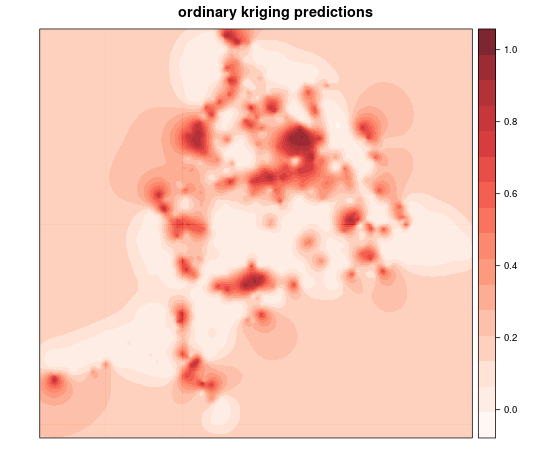
\includegraphics[scale=0.40]{img02}
   \caption{\small{Map of landslide hazards}}
   \label{fig:img02}
  \end{figure}
 \end{center}


\section{Discussion and conclusions}
A landslide hazard assessment study was carried out in Metropolitan Area of San Salvador (MASS). The study started with the construction of a landslide inventory and analysis of the causal factors related to the occurrences of landslide. The problem of modelling landslide generated by different causes is very complex and for this reason the study proved the efficacy of the neural network model with a percentage of correct classification around 80\% against other models such as logistic regression with a percentage of correct classification under 70\%. 

In the process of estimating the weights of the model an heuristic technique was used to obtain a better solution after that a local search was used. It is better than use only backpropagation algorithm or another local search method to estimate weights since that when these are used there is a strong danger of getting stuck in a local minimum rather than a global minimum for a vector of weights.

The problem with the neural network approach is that is difficult to estimate the weights of the model due to intensive computation involved in the present study the estimation of a neural network model takes between 4 and 10 hours for this reason we could not assess the statistical significance of the input variables in the neural network processes using boostrapping. For all of the above parallel computing must be used rather than serial computing in estimating weights of neural networks models.


%%%%  Mencionar abajo las limitaciones computacionales y 
%%%% que no se pudo tomar una muestra mas grande que 1500 
%%%% para el kriging relacionar con lo del big data que puede ser 
%%%% linea de investigación 

The results obtained in the geostatistics methodology showed that the spatial the data satisfies the conditions for applying krigin method. The map of landslide hazard \ref{fig:img02} was generated by krigin method and can be used by non-experts in the landslide phenomenon for many purposes such as territorial planning, prevention and mitigation of natural dissasters and so on. 

Other important variables could not be obtained such as landslide types (Rockfalls, Topples, Slides, etc) and temporal information which can improve the predictive ability of the model. 


\section{Acknowledgment}   
The authors are indebted to M.SC. Giovanni Molina from MARN who provided the data and useful information about landslide modelling techniques.







\begin{thebibliography}{99}


%\bibitem[Carrara(1983)]{Carrara1983403}
\bibitem{Carrara1983403}
Alberto Carrara.
\newblock Multivariate models for landslide hazard evaluation.
\newblock \emph{Journal of the International Association for Mathematical
  Geology}, 15\penalty0 (3):\penalty0 403--426, 1983.
\newblock ISSN 0020-5958.
%\newblock \doi{10.1007/BF01031290}.
\newblock URL \url{http://dx.doi.org/10.1007/BF01031290}.


%\bibitem[Capparelli and P.~Versace(2013)]{hessd-10-12643-2013}
\bibitem{hessd-10-12643-2013}
G.~Capparelli and P.~P.~Versace.
\newblock Landslide susceptibility from mathematical model in sarno area.
\newblock \emph{Hydrology and Earth System Sciences Discussions}, 10\penalty0
  (10):\penalty0 12643--12662, 2013.
%\newblock \doi{10.5194/hessd-10-12643-2013}.
\newblock URL
  \url{http://www.hydrol-earth-syst-sci-discuss.net/10/12643/2013/}.


%\bibitem[Pradhan et~al.(2010)Pradhan, Oh, and
%  Buchroithner]{doi:10.1080/19475705.2010.498151}
\bibitem{doi:10.1080/19475705.2010.498151}
Biswajeet Pradhan, Hyun-Joo Oh, and Manfred Buchroithner.
\newblock Weights-of-evidence model applied to landslide susceptibility mapping
  in a tropical hilly area.
\newblock \emph{Geomatics, Natural Hazards and Risk}, 1\penalty0 (3):\penalty0
  199--223, 2010.
%\newblock \doi{10.1080/19475705.2010.498151}.
\newblock URL
  \url{http://www.tandfonline.com/doi/abs/10.1080/19475705.2010.498151}.
  
  
%\bibitem[Neuhäuser et~al.(2012)Neuhäuser, Damm, and Terhorst]{Neu2012511}
\bibitem{Neu2012511}
Bettina Neuhäuser, Bodo Damm, and Birgit Terhorst.
\newblock Gis-based assessment of landslide susceptibility on the base of the
  weights-of-evidence model.
\newblock \emph{Landslides}, 9\penalty0 (4):\penalty0 511--528, 2012.
\newblock ISSN 1612-510X.
%\newblock \doi{10.1007/s10346-011-0305-5}.
\newblock URL \url{http://dx.doi.org/10.1007/s10346-011-0305-5}.



%\bibitem[Bernknopf and Shapiro(1988)]{Bern198839}
\bibitem{Bern198839}
Campbell R.H. Brookshire~D.S. Bernknopf, R.L. and C.D Shapiro.
\newblock A probabilistic approach to landslide hazard mapping in cincinnati,
  ohio, with application for economic evaluation.
\newblock \emph{Bulletin of the Association of Engineering Geologists},
  XXV\penalty0 (1):\penalty0 39--56, 1988.
  
  
%\bibitem[Chung and Fabbri(2003)]{Chung2003451}
\bibitem{Chung2003451}
Chang-JoF. Chung and AndreaG. Fabbri.
\newblock Validation of spatial prediction models for landslide hazard mapping.
\newblock \emph{Natural Hazards}, 30\penalty0 (3):\penalty0 451--472, 2003.
\newblock ISSN 0921-030X.
%\newblock \doi{10.1023/B:NHAZ.0000007172.62651.2b}.
\newblock URL \url{http://dx.doi.org/10.1023/B\%3ANHAZ.0000007172.62651.2b}.  

%\bibitem[Lee et~al.(2004)Lee, Choi, and Min]{doi:10.1080/01431160310001618734}
\bibitem{doi:10.1080/01431160310001618734}
S.~Lee, J.~Choi, and K.~Min.
\newblock Probabilistic landslide hazard mapping using gis and remote sensing
  data at boun, korea.
\newblock \emph{International Journal of Remote Sensing}, 25\penalty0
  (11):\penalty0 2037--2052, 2004.
%\newblock \doi{10.1080/01431160310001618734}.
\newblock URL
  \url{http://www.tandfonline.com/doi/abs/10.1080/01431160310001618734}.

%\bibitem[Melchiorre et~al.(2011)Melchiorre, Abella, van Westen, and
%  Matteucci]{Melchiorre2011410}
\bibitem{Melchiorre2011410}
C.~Melchiorre, E.A.~Castellanos Abella, C.J. van Westen, and M.~Matteucci.
\newblock Evaluation of prediction capability, robustness, and sensitivity in
  non-linear landslide susceptibility models, guantánamo, cuba.
\newblock \emph{Computers {\&} Geosciences}, 37\penalty0 (4):\penalty0 410 --
  425, 2011.
\newblock ISSN 0098-3004.
%\newblock \doi{http://dx.doi.org/10.1016/j.cageo.2010.10.004}.
\newblock URL
  \url{http://www.sciencedirect.com/science/article/pii/S0098300410003286}.

%\bibitem[Zeng-wang(2001)]{Zeng2001374}
\bibitem{Zeng2001374}
Xu~Zeng-wang.
\newblock Gis and ann model for landslide susceptibility mapping.
\newblock \emph{Journal of Geographical Sciences}, 11\penalty0 (3):\penalty0
  374--381, 2001.
\newblock ISSN 1009-637X.
%\newblock \doi{10.1007/BF02892323}.
\newblock URL \url{http://dx.doi.org/10.1007/BF02892323}.


%\bibitem[Erm(2005)]{Ermini2005327}
\bibitem{Ermini2005327}
Artificial neural networks applied to landslide susceptibility assessment.
\newblock \emph{Geomorphology}, 66\penalty0 (1–4):\penalty0 327 -- 343, 2005.
\newblock ISSN 0169-555X
%\newblock \doi{http://dx.doi.org/10.1016/j.geomorph.2004.09.025}.
\newblock URL \url{http://www.sciencedirect.com/science/article/pii/S0169555X04002272}.



\bibitem{Yesilnacar2005251}
E. Yesilnacar and T. Topal.
\newblock Landslide susceptibility mapping: A comparison of logistic regression and neural networks methods in a medium scale study, Hendek region (Turkey).
\newblock \emph{Engineering Geology}, 79\penalty0
  (11):\penalty0 251-266, 2005.
\newblock ISSN 0013-7952,
%\newblock \doi{10.1080/01431160310001618734}.
\newblock URL
  \url{http://www.sciencedirect.com/science/article/pii/S0013795205000384}.


\bibitem{McNelis2005}
Paul D. McNelis
\newblock Estimation of a Network with Evolutionary Computation
\newblock \emph{Academic Press},
  (11):\penalty0 59-84, 2005.
\newblock ISBN 9780124859678,
%\newblock \doi{http://dx.doi.org/10.1016/B978-012485967-8.50003-8}.
\newblock URL
  \url{http://www.sciencedirect.com/science/article/pii/B9780124859678500038}.



\bibitem{FAQANN}
Warren S. Sarle
\newblock URL
  \url{ftp://ftp.sas.com/pub/neural/FAQ.html#questions}.
  \newblock Accessed 31 May, 2015.


\bibitem{ballabio2012support}
Ballabio, Cristiano and Sterlacchini, Simone
\newblock Support vector machines for landslide susceptibility mapping: the Staffora River Basin case study, Italy
\newblock \emph{Mathematical geosciences},
  (11):\penalty0 1, 47--70, 2012.
\newblock Springer. 



\bibitem{tien2012landslide}
Tien Bui, Dieu and Pradhan, Biswajeet and Lofman, Owe and Revhaug, Inge
\newblock Landslide susceptibility assessment in vietnam using support vector machines, decision tree, and Naive Bayes Models
\newblock \emph{Mathematical Problems in Engineering},
  (11):\penalty0 2012, 2012.
\newblock Hindawi Publishing Corporation.



\bibitem{akgun2012}
Akgun, Aykut
\newblock A comparison of landslide susceptibility maps produced by logistic regression, multi criteria decision, and likelihood ratio methods: a case study at Izmir, Turkey
\newblock \emph{Landslides},
  (11):\penalty0 9, 1, 93--106, 2012
\newblock Springer. 


\bibitem{gaskill}
Gaskill, Jacob and Zuber, Brian and Nordman, Erik
\newblock Analyzing Landslide Susceptibility in St. Vincent and the Grenadines Using Co-Kriging and Logistic Regression
\newblock \emph{The 2015 IMAGIN Award, Michigan United States}.
\newblock URL
  \url{http://www.imagin.org/awards/sppc/2015/papers/jacob_gaskill_paper.pdf}.


\bibitem{van2006landslide}
Van Westen, CJ and Van Asch, Th WJ and Soeters, R
\newblock Landslide hazard and risk zonation why is it still so difficult?
\newblock \emph{Bulletin of Engineering geology and the Environment}.
(65):\penalty0 2, 167--184, 2006
\newblock Springer. 







\end{thebibliography}

\end{document}

